\documentclass[12pt]{article}
\usepackage{amsmath, amssymb, amsthm}
\usepackage{geometry}
\usepackage{hyperref}
\usepackage{listings}
\usepackage{xcolor}
\usepackage{graphicx}
\usepackage{booktabs}
\usepackage{array}
\usepackage{tikz}
\usetikzlibrary{arrows.meta, positioning}
\definecolor{stageblue}{HTML}{307BF3}

\geometry{margin=1in}

\lstset{
    language=Python,
    basicstyle=\ttfamily\small,
    keywordstyle=\color{blue},
    stringstyle=\color{red},
    commentstyle=\color{green!50!black},
    showstringspaces=false,
    breaklines=true,
    frame=single,
    numbers=left,
    numberstyle=\tiny
}

\title{Special Topics in Applied Mathematics I \\ Solution 2}
\author{XIA JIAHAN}
\date{\today}

\begin{document}
\maketitle

\section{Introduction to Recommendation Systems}

In the information explosion era, recommendation systems (RS) are essential for filtering vast data and delivering personalized content across platforms like Amazon, Netflix, YouTube, and social media, enhancing user experience and business value by predicting preferences. They use machine learning to model similarities between items and user interests, powering two main types of suggestions: personalized homepage feeds (unique to each user) and related item recommendations (e.g., suggesting science apps when viewing a math app). This enables platforms like YouTube and the Google Play Store to anticipate what to show next. The core motivation is to help users navigate immense content libraries, where search alone falls short, by surfacing relevant, sometimes unexpected items and facilitating discovery.

A recommender system matches a user's query (context) to recommendable entities (items) by learning embeddings that place queries and items in a shared vector space for efficient similarity computation. It then performs candidate generation to quickly narrow a huge corpus to hundreds or thousands of candidates, scoring to rank this smaller set and select roughly ten items to display, and finally re-ranking to apply constraints such as removing content the user dislikes, boosting fresher items, and ensuring diversity and fairness. We will discuss each stage with examples from systems like YouTube.

\begin{figure}[htbp]
    \centering
    \resizebox{\linewidth}{!}{%
    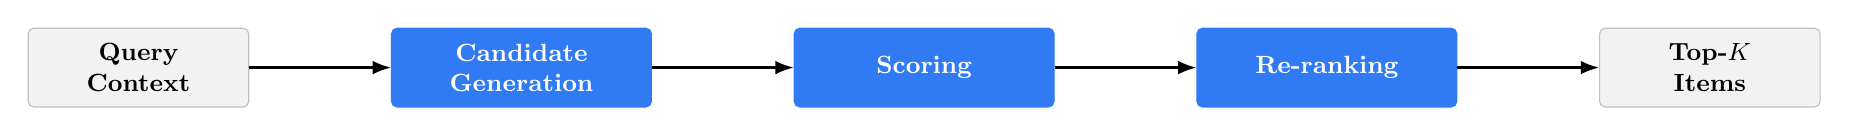
\begin{tikzpicture}[
        node distance=1.8cm,
        >=Latex,
        stage/.style={draw=stageblue, fill=stageblue, rounded corners=2pt, text=white, font=\small\bfseries, minimum height=10mm, minimum width=33mm, align=center},
        io/.style={draw=black!25, fill=black!5, rounded corners=2pt, font=\small\bfseries, minimum height=10mm, minimum width=28mm, align=center}
    ]
        \node[io] (query) {Query\\Context};
        \node[stage, right=of query] (cand) {Candidate\\Generation};
        \node[stage, right=of cand] (score) {Scoring};
        \node[stage, right=of score] (rerank) {Re-ranking};
        \node[io, right=of rerank] (results) {Top-$K$\\Items};

        \draw[->, thick] (query) -- (cand);
        \draw[->, thick] (cand) -- (score);
        \draw[->, thick] (score) -- (rerank);
        \draw[->, thick] (rerank) -- (results);
    \end{tikzpicture}%
    }
    \caption{Overview of the Recommender System Process}
    \label{fig:process_flow}
\end{figure}


\end{document}
